\section[1D models of vibrations]{\hyperlink{toc}{1D models of vibrations}}

\begin{itemize}
    \item monatomic chain (restricted to longitudinal motion for now.)
    \item a: lattice constant and k: spring constant
    \item equilibrium position for the nth atom and displacement.
    \[x_n^{eq}= na\]
    \[\delta x_n = x_n - x_n^{eq}\]
    \item Hooke's Law:
    \[F_n = k( \delta x_{n+1} - \delta x_n)-k(\delta x_n - \delta x_{n-1})\]
    \item Newton's Law $\rightarrow$ equations of motion (EoM) make ansatz:
    \[\delta x_n = A e^{-ikna + i \omega t} \] 
    \item Plug ansatz into Newton:
    \[ \omega = 2 \sqrt{\frac{k}{m}\left| \sin\left(\frac{ka}{2}\right)\right|} \]
    \item A: amplitude and k: wave vector (related to momentum).
    \item Point with k=0; Reciprical Lattice points $G_m$ and Positions of atoms of along the chain $x_n$.
    \[G_n = \frac{2 \pi n}{a} , \qquad n = -2,-1,0,1,2,...\]
    \item Reciprocal lattice $\leftrightarrow$ Direct lattice
    \item
    \[e^{iG_m x_n} = 1 \]
    \item 1st Brillouin Zone: unit cell centered around k=0 with boundaries @ $k= \pm \frac{\pi}{a}$ in reciprocal lattice. All allowed cases contained in 1st. 2nd 3rd etc can be helpful but not needed.
    \item for finite length: 
    \[k=\frac{2\pi n}{L} \] 
    \textbf{Phonons}
    \[E_n = (\frac{1}{2}+n)h\omega \]
    \item each excitation of harmonic oscillators corresponding to vibrations in a material $\rightarrow$ bosons (which phonons are).
    
    \item number of phonons is $\therefore$ given by Bose distribution.
    \[n_B (\beta \hbar\omega) = \frac{1}{e^{\beta \hbar\omega} -1 } \]
    \item Diatomic chain + excitations with multiple branches
    $\rightarrow$ leads to increase in possible modes of vibrations.
    \item Again assume coupled according to Hooke's Law (and easier if we let m1=m1)
    \item Sol. Newton:
    \[\begin{cases}
      m \frac{d^2(\delta x_n)}{\partial t^2} = k_2 (\delta y_n - \delta x_n)+ k_1 (\delta y_{n-1} - \delta x_n)\\
      m \frac{d^2(\delta y_n)}{\partial t^2} = k_2 (\delta x_n - \delta y_n)+ k_1 (\delta x_{n} - \delta y_n)
    \end{cases} \]
    \item Ansatz:Plug into the matrix form of EoM.
    \[\begin{cases}
    \delta x_n = A_x e^{-ikna+i\omega t} \\
    \delta y_n = A_y e^{-ikna+i\omega t}
    \end{cases}\]
    \item solve for $\omega$. plus or minus solutions or multiple solutions will give a E-k diagram and thus the Single Brillouin Zone. The top one in this case is Optical phonons and the bottom is Acoustic phonons (which are nuanced names. Photons can interact only with the "optical" phonons. 
    \[\omega = 2 \sqrt{\frac{k}{m}} \left| \sin\left(\frac{ka}{2}\right)\right| \]
    \begin{figure}
        \centering
        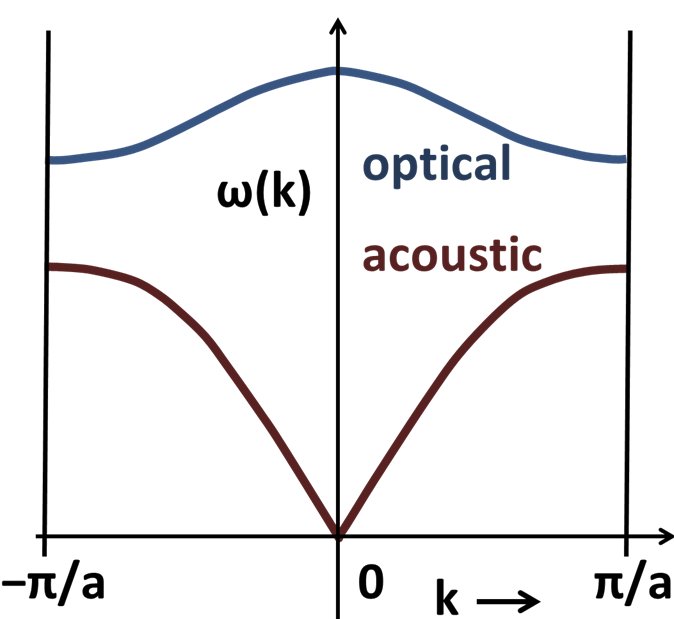
\includegraphics[width = 0.5\linewidth]{Images/phonon_modes.png}
        \caption{Caption}
        \label{fig:phonon modes}
    \end{figure}
    \item \textbf{Extended zone scheme}
    \begin{itemize}
        \item shifts the optical to the second brillouin zone and leaves the acoustic in the first.
        \item makes it easier to see the change from diatomic to monatomic.
        \begin{figure}
            \centering
            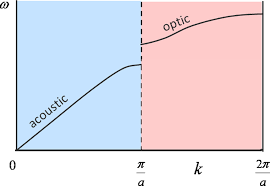
\includegraphics[width = 0.5\linewidth]{Images/extended_zone_scheme.png}
            \caption{extended zone scheme}
            \label{fig:extended zone scheme}
        \end{figure}
    \end{itemize}
\end{itemize}

